% report.tex
% Report.
% Copyright (C) 2010 Vladimir Rutsky <altsysrq@gmail.com>

% TODO: Use styles according to GOST (it's hard).

\documentclass[a4paper,10pt]{article}

% Encoding support.
\usepackage{ucs}
\usepackage[utf8x]{inputenc}
\usepackage[T2A]{fontenc}
\usepackage[russian]{babel}

\usepackage{amsmath, amsthm, amssymb}

% Indenting first paragraph.
\usepackage{indentfirst}

\usepackage{url}
\usepackage[unicode]{hyperref}

%\usepackage[final]{pdfpages}

\usepackage[pdftex]{graphicx}
\usepackage{subfig}

\newcommand{\HRule}{\rule{\linewidth}{0.5mm}}

% Spaces after commas.
\frenchspacing
% Minimal carrying number of characters,
\righthyphenmin=2

% From K.V.Voroncov Latex in samples, 2005.
\textheight=24cm   % text height
\textwidth=16cm    % text width.
\oddsidemargin=0pt % left side indention
\topmargin=-1.5cm  % top side indention.
\parindent=24pt    % paragraph indent
\parskip=0pt       % distance between paragraphs.
\tolerance=2000
%\flushbottom       % page height aligning
%\hoffset=0cm
%\pagestyle{empty}  % without numeration

\newcommand{\myemail}[1]{%
\href{mailto:#1}{\nolinkurl{#1}}}

\begin{document}

% Title page.
% title.tex
% Report title page.
% Copyright (C) 2010 Vladimir Rutsky <altsysrq@gmail.com>

\begin{titlepage} % начало титульной страницы

\begin{center} % включить выравнивание по центру

\large Санкт-Петербургский государственный политехнический университет\\[4.5cm]
% название института, затем отступ 4,5см

\huge Отчет по лабораторной работе \No 1\\[0.6cm] % название работы, затем отступ 0,6см
\large по~курсу <<Компьютерная графика>>\\[1cm]
\large <<Представление криволинейной поверхности координатной сеткой 
с удалением невидимых линий методом плавающего горизонта>>\\[3.7cm]
% тема работы, затем отступ 3,7см

\begin{flushright} % выровнять её содержимое по левому краю
\begin{tabular}{l l}
\emph{Студент:} & Руцкий~В.\,В.\\
\emph{Группа:} & 4057/2\\
\emph{Преподаватель:} & Ильин~Ю.\,П.
\end{tabular}
\end{flushright} % конец выравнивания по левому краю

\vfill % заполнить всё доступное ниже пространство

{\large Санкт-Петербург 2010}
\end{center} % закончить выравнивание по центру
\thispagestyle{empty} % не нумеровать страницу
\end{titlepage} % конец титульной страницы


% Content

\section{Задание}
Требуется модифицировать базовый пакет для создания фотореалистичных изображений трёхмерных сцен 
методом обратной трассировки лучей из \cite{shikin1995cg} (в дальнейшем именуемый <<пакет>>),
и добавить в него эффект дисперсии света при преломлении.

\section{Описание метода}
Рассмотрим физическую основу цвета.

Луч света представляет собой композицию волн разных длин.
Распределение количества волн по их длинам задаёт то, 
как этот луч света будет восприниматься наблюдателем, 
каким \textit{цветом} он будет видеть этот луч.
Диффузные или полупрозрачные объекты отражают или пропускают через себя волны лишь определённых длин,
в результате, наблюдатель видит объект определённого цвета, а не цвета источника света.

В используемой модели можно считать, 
что световые волны распространяются независимо друг от друга, 
поэтому можно разбить исходный диапазон длин волн источников 
на несколько непересекающихся групп диапазонов $g_1, \ldots, g_n$, 
осветить сцену по отдельности лучами из диапазонов разбиения~--- 
полученный набор изображений $I_1, \ldots, I_n$ будет содержать только цвета, 
соответствующие длинам волн $g_1, \ldots, g_n$, 
затем объеденить изображения $I_1, \ldots, I_n$ в результирующее изображение.

Дисперсия света~--- явление зависимости абсолютного показателя преломления вещества от длины волны света.
В результате дисперии света волны разной длины исходящие вдоль одного луча от источника света 
распространяются по разному.

Идея моделирования эффекта дисперсии света состоит в следующем.
Ограничим исходный набор длин волн источников трёмя составляющими $r$, $g$ и $b$~---
волнами, соответствующими красному, синему и зеленому цветам.
Построим три изображения сцены $I_r, I_g, I_b$, соответствующие
освещению только лучами с длинами волн взятых составляющих $r$, $g$ и $b$.
Так как изображения сцены $I_r, I_g, I_b$ строятся для определённых длин волн, 
при их построении для объектов сцены можно использовать показатели преломления соответствующие длинам
проходящих через них волн.
Тогда после объединения $I_r, I_g, I_b$ результирующее изображение будет учитывать дисперсию света для
основных составляющих $r$, $g$ и $b$.

\subsection{Детали реализации}
В исходной реализации метода трассировки лучей для каждого светопропускающего материала указывается 
величина абсолютного показателя преломления вещества, которая используется для рассчета угла преломления.

Для реализации эффекта дисперсии света, 
для каждого светопропускающего материала была указана величина абсолютного показателя преломления вещества для волн,
соответствующих взятым компонентам $r$, $g$ и $b$.
При первом преломлении производится разделение исходного луча на три луча, соответствующие $r$, $g$ и $b$.
При запуске луча, преломлённого полупрозрачным объектом, 
направление преломления выбирается в зависимости от обрабатываемой в данный момент компоненты.

Для увеличения реалистичности получаемых изображения был дополнительно реализован 
эффект полного внутреннего отражения.

\paragraph{Внесённые изменения}
Исходный пакет был написан в 1995 году для ОС \textit{DOS} и для сборки в компиляторе \textit{Turbo C++}%
%\footnote{\textit{Turbo C++} версии для \textit{DOS} и \textit{Microsoft Windows 3.11}~--- 
%более не разрабатываемый компилятор и интегрированная среда разработки для C++ от компании \textit{Borland}}%
.
Для удобства разработки и отладки пакет был портирован в современные ОС.

Для сборки в среде GNU/Linux использолись средства \textit{GCC}%
\footnote{\textit{GNU Compiler Collection}, \url{http://gcc.gnu.org/}} 
(использовалась версия 4.4.3) вместе с \textit{SCons}%
\footnote{свободный инструмент для автоматизации сборки программных пакетов, \url{http://scons.org/}} 
(версии 1.2.0) и
\textit{Eclipse}%
\footnote{свободная интегрированная среда разработки, \url{http://eclipse.org/}} 
(версии 3.5.2) с плагином для разработки приложений на C++ \textit{Eclipse CDT}%
\footnote{\textit{Eclipse CDT (C/C++ Development Tooling)}, \url{http://www.eclipse.org/cdt/}}
(версии 6.0.2);
для сборки в среде Windows~--- \textit{Microsoft Visual Studio}%
\footnote{\url{http://www.microsoft.com/visualstudio}}
(использовалась бесплатная версия \textit{Microsoft Visual C++ 2008 Express Edition} c SP1).

Были внесены следующие существенные изменения:
\begin{enumerate}
  \item Удалён модуль, отвечающий за отрисовку изображения на экране во время построения изображения (\textit{draw.cpp}, \textit{draw.h}), 
  ввиду отстутствия необходимости в нём и невозможности работы исходной версии для DOS в GNU/Linux.
  \item Ввод/вывод изображений был переписан с использованием свободной библиотеки \textit{Boost.GIL}%
\footnote{Generic Image Library, \url{http://www.boost.org/doc/libs/1_44_0/libs/gil/doc/index.html}} 
(удалены модули \textit{bmp.cpp}, \textit{bmp.h}, \textit{targa.cpp}, \textit{targa.h}; 
добавлены модули \textit{image.cpp}, \textit{image.h}, \textit{rgb.h})
  \item Исправлены конструкции языка С++ недопустимые в новым стандарте языка.
  \item Добавлен заголовочный файл для предварительной компиляции \textit{precompiled.h}.
  \item Разбит модуль \textit{tracer.cpp} на несколько модулей согласно выполняемым функциям:
  \textit{gobject.cpp}, \textit{gobject.h}, \textit{lightsource.h}, \textit{mapping.h}, 
  \textit{medium.cpp}, \textit{medium.h}, \textit{surfacedata.h}.
  \item Глобальные переменные, описывающие сцену, были инкапсулированы в класс \textit{Environment} (\textit{tracer.cpp}).
  \item Обработка преломления света была вынесена в отдельную функцию \textit{Environment::handleRefraction} (\textit{tracer.cpp}).
  \item В функцию вычисления освещённости точки \textit{shadeImpl} (в оригинальном пакете она называлась \textit{Shade}) 
  были внесены описанные выше изменения по поддержке эффекта дисперсии света и эффекта полного внутреннего отражения.
\end{enumerate}
Полная история изменений доступна в виде лога системы контроля версий \textit{git}%
\footnote{свободная распределённая система управления версиями файлов, \url{http://git-scm.com/}}
на сайте проекта по адресу \url{http://sourceforge.net/p/braytracing/git/ref/master\%3A/log/}.

\subsection{Проверка корректности}
Для проверки корректности работы программы одна и та же сцена была построена в разрабатываемой программе и
трёхмерном редакторе \textit{Blender}%
\footnote{\textit{Blender}~--- свободный пакет для создания трёхмерной компьютерной графики, \url{http://www.blender.org/}}.
\begin{figure}[h!]
  \centering
  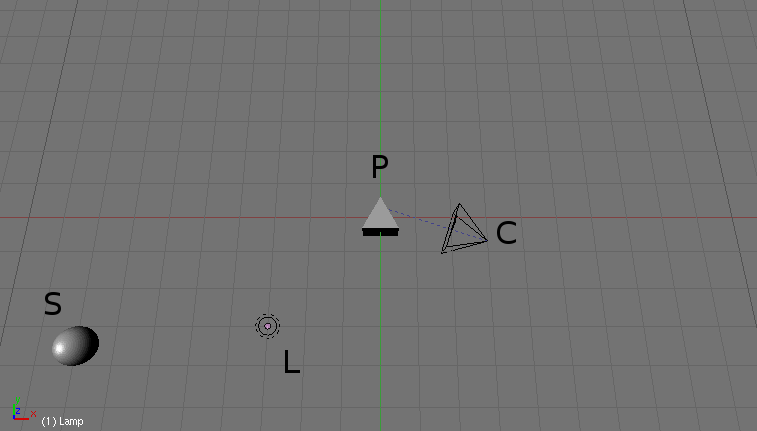
\includegraphics[width=0.8\linewidth]{./screenshots/prism_test_model.png}
  \caption{Модель тестовой сцены}
  \label{fig:prism-test-model}
\end{figure}
В качестве тестовой сцены была взята сцена, изображенная на рис.~\ref{fig:prism-test-model}: 
наблюдатель $C$ справа смотрит на прозрачную треугольную призму $P$ в центре сцены,
через призму, в результате преломления к основанию, видна сфера $S$, освещённая источником света $L$.

Из-за особенностей реализации исходного пакета, не получится наблюдать через призму источник света напрямую~---
требуется, чтобы была освещаемая поверхность, для этого и была введена освещённая сфера $S$.

Результат моделирования сцены в модифицированном пакете приведён на рис.~\ref{fig:prism-test-brt},
а результат моделирования в \textit{Blender} на рис.~\ref{fig:prism-test-blender} 
(в стандартной комплектации \textit{Blender} нет поддержки эффекта дисперсии света при преломлении).
\begin{figure}
  \centering
  %\subfloat[Рендеринг в пакете]{\label{fig:prism-test-brt}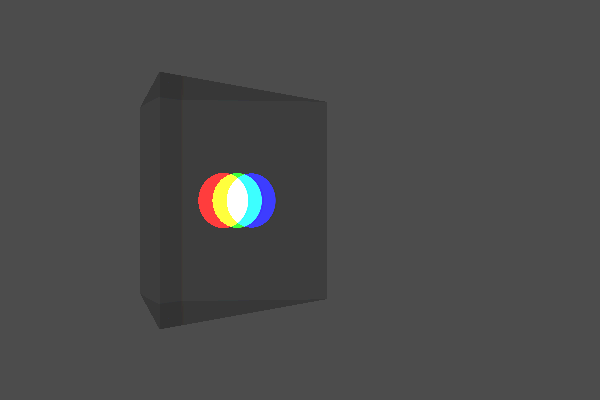
\includegraphics[width=0.3\textwidth]{./screenshots/prism_test_brt.png}}
  \subfloat[Рендеринг в пакете]{\label{fig:prism-test-brt}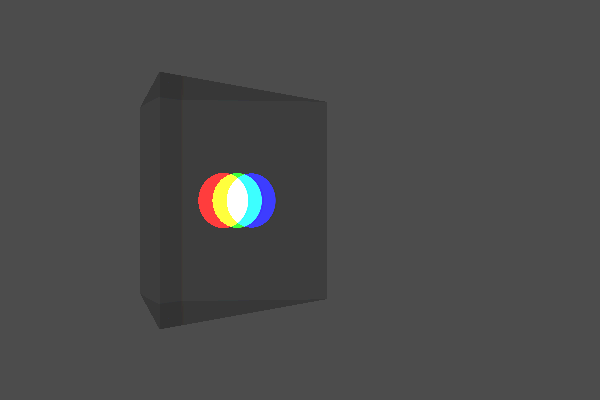
\includegraphics[height=5cm]{./screenshots/prism_test_brt.png}}
  \quad
  %\subfloat[Рендеринг в \textit{Blender}]{\label{fig:prism-test-blender}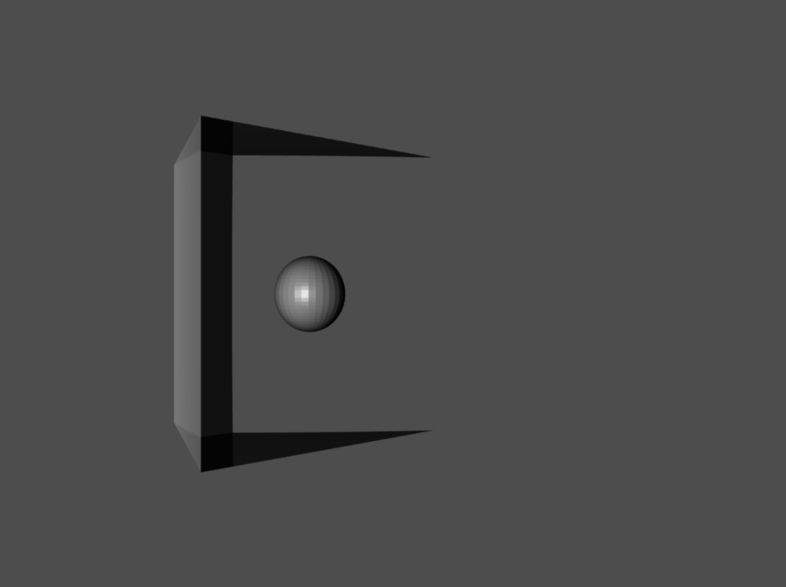
\includegraphics[width=0.3\textwidth]{./screenshots/prism_test_blender.png}}
  \subfloat[Рендеринг в \textit{Blender}]{\label{fig:prism-test-blender}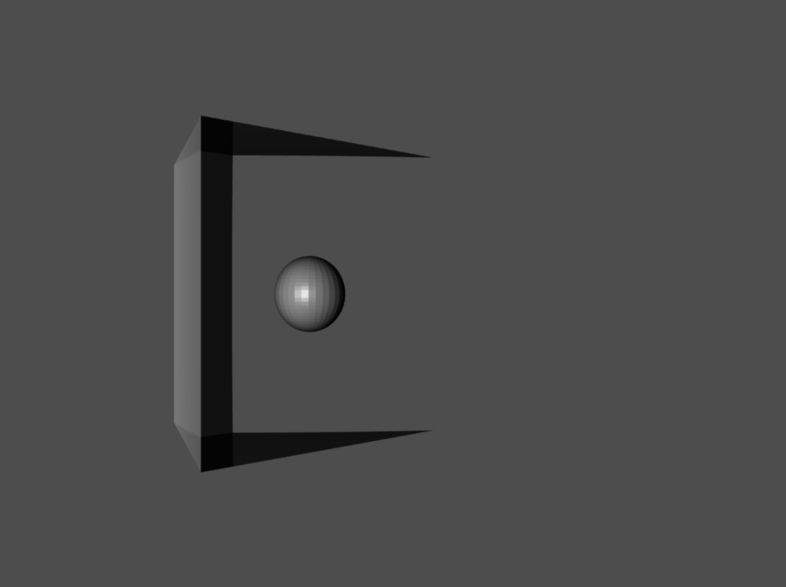
\includegraphics[height=5cm]{./screenshots/prism_test_blender.png}}
  \caption{Рендеринг тестовой сцены}
  \label{fig:prism-test-results}
\end{figure}

На изображениях видно, что преломлённая сфера находится примерно в одном месте, 
что показывает корректность рассчета величины преломления.

Так как наблюдается неточечный источник света через призму,
а не результат разложения узкого пучка света в призме, 
на результирующем изображении должна получиться <<радуга>> с обратным порядком цветов, 
что наблюдается на рис.~\ref{fig:prism-test-brt}.

\section{Результат работы}
Рендеринг модели алмаза в пакете и \textit{Blender} приведён на рис.~\ref{fig:diamond-brt} и \ref{fig:diamond-blender} соответственно.
На изображениях виден результат множественного внутреннего отражения и изменение цвета в результате эффекта дисперсии.

С разрешения автора%
\footnote{Алексей~В.\,Боресков \myemail{steps3d@narod.ru}, \myemail{steps3d@gmail.com}}
оригинальные и модифицированные исходные коды пакета распространяются под свободной лицензией~--- GNU GPL%
\footnote{GNU General Public License, \url{http://www.gnu.org/licenses/gpl.html}} версии 3. 
Проект расположен на хостинге для открытого ПО SourceForge.net\footnote{\url{http://sourceforge.net}} по адресу
\url{http://sourceforge.net/p/braytracing/}.

\begin{figure}
  \centering
  \subfloat[Рендеринг в пакете]{\label{fig:diamond-brt}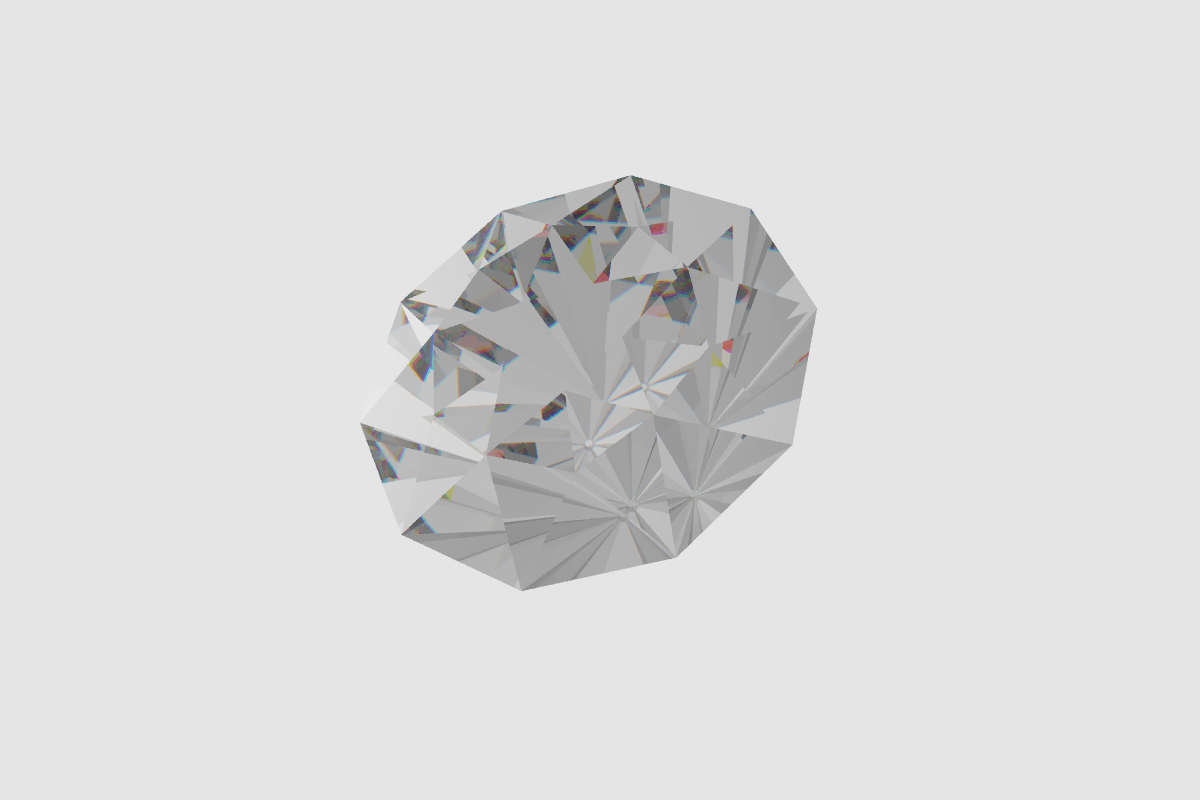
\includegraphics[width=0.8\textwidth]{./screenshots/diamond_brt.png}}
  \\
  \subfloat[Рендеринг в \textit{Blender}]{\label{fig:diamond-blender}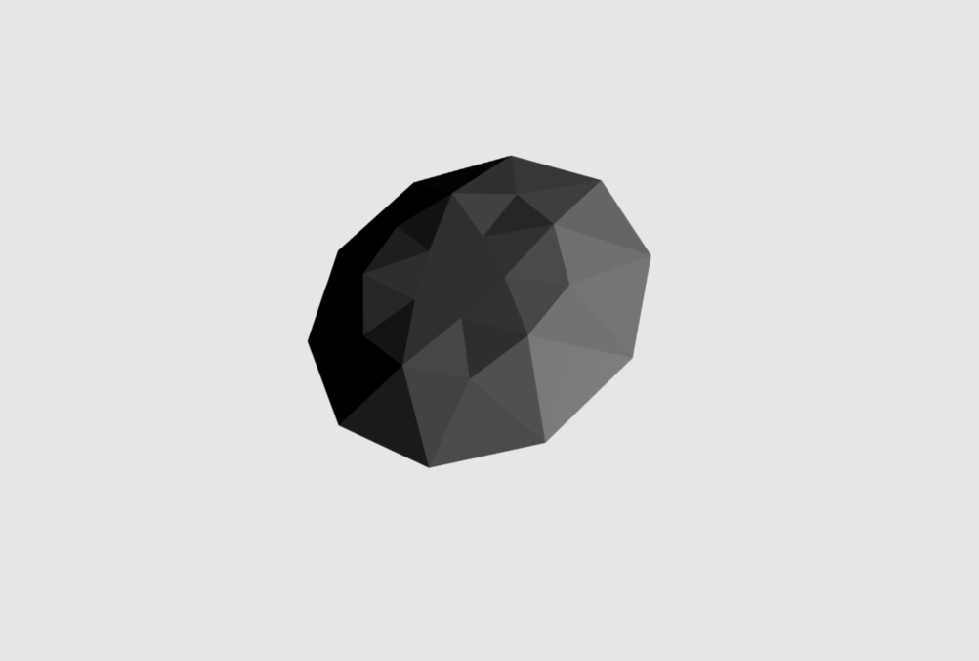
\includegraphics[width=0.8\textwidth]{./screenshots/diamond_blender.png}}
  \caption{Рендеринг модели алмаза}
  \label{fig:diamond-results}
\end{figure}

\bibliographystyle{unsrt}
\bibliography{references.bib}

\end{document}
